%! Author = Omar Iskandarani
%! Title = The Vortex Æther Model: A Unified Topological Field Theory of Mass, Gravity, and Time
%! Date = ...
%! Affiliation = Independent Researcher, Groningen, The Netherlands
%! License = CC-BY 4.0
%! ORCID = 0009-0006-1686-3961
%! DOI = ..

\newcommand{\paperdoi}{...}
\documentclass[12pt,aps,prd,onecolumn,nofootinbib,superscriptaddress]{revtex4-2}

% ==================== Packages ====================
\usepackage[utf8]{inputenc}
\usepackage[T1]{fontenc}
\usepackage{lmodern}
\usepackage{amsmath,amssymb,amsfonts}
\usepackage{graphicx}
\usepackage{hyperref}
\usepackage{doi}
\usepackage{physics}
\usepackage{mathtools}
\usepackage{tikz}
\usetikzlibrary{knots,intersections,decorations.pathreplacing}
\usetikzlibrary{3d, calc, arrows.meta, positioning}
\usepackage{pgfmath}
\usetikzlibrary{decorations.pathmorphing}
\usepackage{pgfplots}
\pgfplotsset{compat=1.18} % or version you have
\usepackage{bm}          % bold math
\usepackage{titlesec}    % section formatting (optional)
\usepackage{float}       % [H] float placement
\newcommand{\knotgif}[1]{\includegraphics[height=1.2em]{images/#1.gif}}
% ==================== Metadata ====================
\begin{document}

\title{The Vortex Æther Model: \\[1ex]
        \large A Unified Topological Field Theory of Mass, Gravity, and Time}

\author{Omar Iskandarani}
\email{info@omariskandarani.com}
\affiliation{Independent Researcher, Groningen, The Netherlands}
\thanks{ORCID: \href{https://orcid.org/0009-0006-1686-3961}{0009-0006-1686-3961}}
\thanks{DOI: \href{https://doi.org/\paperdoi}{\paperdoi}}
\thanks{License: CC-BY 4.0 International}
    
\date{\today}

% ==================== Abstract ====================
\begin{abstract}
            We present the Vortex Æther Model (VAM), a unified physical framework in which mass, gravity, and proper time emerge from topologically structured vorticity within a compressible, inviscid æther. In contrast to curvature-based relativity and Higgs-based mass generation, VAM describes particles as knotted vortex excitations, and gravity as a swirl-induced time deviation field. The theory reproduces classical phenomena such as gravitational redshift, time dilation, and frame-dragging through fluid-dynamic energetics, and calculates particle masses and physical constants from first principles. The Standard Model gauge groups SU(3), SU(2), and U(1) arise naturally from vortex topology and swirl symmetry, while canonical quantization defines a Fock-like Hilbert space over knot eigenstates. We develop a full path-integral formulation over topological sectors of the æther manifold, enabling quantum transitions, knot fusion, and helicity exchange interactions. Benchmarking against general relativity and experimental tests of gravitational time deviation support the model’s viability. VAM offers a physically grounded, falsifiable, and derivational alternative to conventional quantum gravity and field theory models.
\end{abstract}
\maketitle

        \begin{figure}[H]
            \centering
            \footnotesize
            \scalebox{0.75}{
                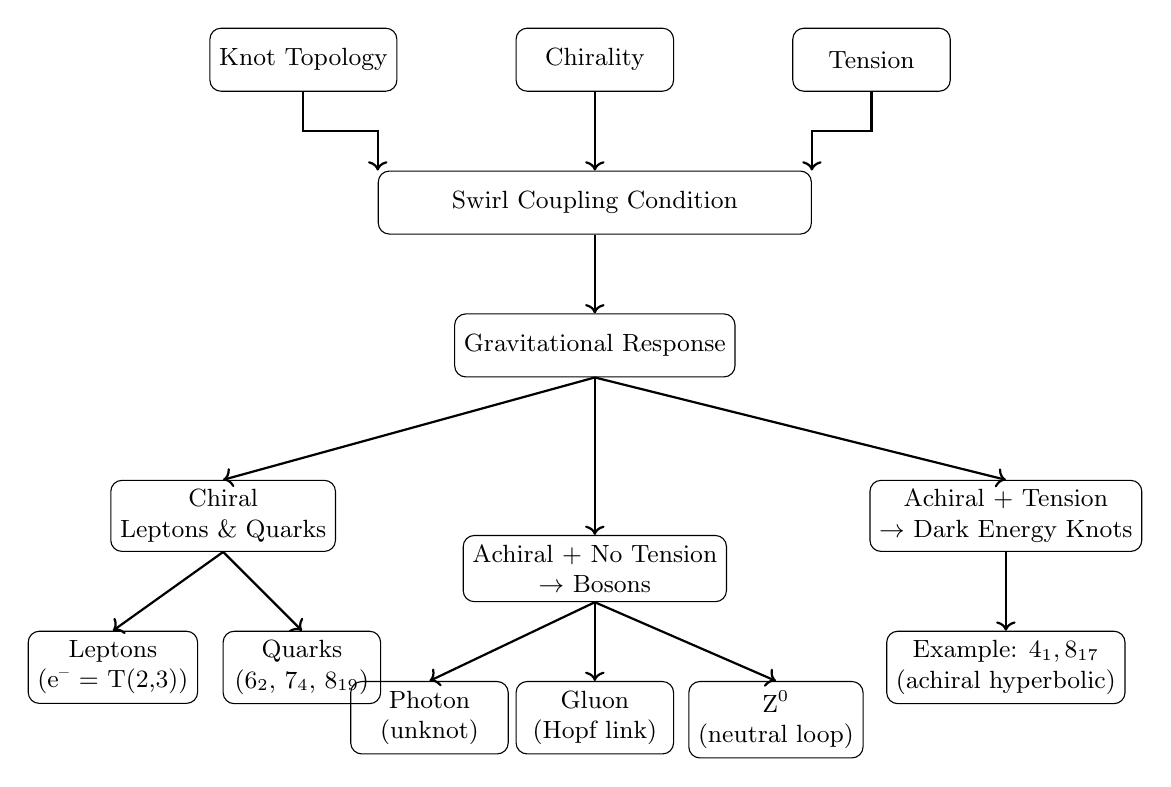
\begin{tikzpicture}[
                  box/.style = {draw, rounded corners, minimum width=2.0cm, minimum height=0.8cm, font=\small, align=center},
                  arrow/.style = {->, thick},   node distance=1.0cm and 1.5cm
                ]
                    % Inputs
                    \node[box] (topology) {Knot Topology};
                    \node[box, right=of topology] (chirality) {Chirality};
                    \node[box, right=of chirality] (tension) {Tension};

                    % Swirl coupling
                    \node[box, below=of chirality, minimum width=5.5cm] (coupling) {Swirl Coupling Condition};

                    % Gravitational response
                    \node[box, below=of coupling] (grav) {Gravitational Response};

                    % Gravitational classes
                    \node[box, below left=1.3cm and 1.5cm of grav] (matter) {Chiral\\Leptons \& Quarks};
                    \node[box, below=2cm of grav] (boson) {Achiral + No Tension\\\(\rightarrow\) Bosons};
                    \node[box, below right=1.3cm and 1.7cm of grav] (dark) {Achiral + Tension\\\(\rightarrow\) Dark Energy Knots};

                    % Subclasses
                    \node[box, below=of matter, xshift=-1.4cm] (leptons) {Leptons\\(e\textsuperscript{--} = T(2,3))};
                    \node[box, below=of matter, xshift=+1.0cm] (quarks) {Quarks\\(6\textsubscript{2}, 7\textsubscript{4}, 8\textsubscript{19})};

                    \node[box, below=of boson, xshift=-2.1cm] (photon) {Photon\\(unknot)};
                    \node[box, below=of boson] (gluon) {Gluon\\(Hopf link)};
                    \node[box, below=of boson, xshift=+2.3cm] (zboson) {Z\textsuperscript{0}\\(neutral loop)};

                    \node[box, below=of dark] (darkex) {Example: \(4_{1}, 8_{17}\)\\ (achiral hyperbolic)};

                    % Arrows to coupling
                    \draw[arrow] (topology.south) -- ++(0,-0.5) -| (coupling.north west);
                    \draw[arrow] (chirality.south) -- (coupling.north);
                    \draw[arrow] (tension.south) -- ++(0,-0.5) -| (coupling.north east);

                    % Arrows down flow
                    \draw[arrow] (coupling.south) -- (grav.north);
                    \draw[arrow] (grav.south) -- (matter.north);
                    \draw[arrow] (grav.south) -- (boson.north);
                    \draw[arrow] (grav.south) -- (dark.north);

                    % Particle branches
                    \draw[arrow] (matter.south) -- (leptons.north);
                    \draw[arrow] (matter.south) -- (quarks.north);

                    \draw[arrow] (boson.south) -- (photon.north);
                    \draw[arrow] (boson.south) -- (gluon.north);
                    \draw[arrow] (boson.south) -- (zboson.north);

                    \draw[arrow] (dark.south) -- (darkex.north);
                \end{tikzpicture}
            }
            \caption{Knot Classification by Swirl Coupling.
                The flowchart visualizes how knot topology, chirality, and curvature tension determine gravitational behavior, and how this leads to specific particle subclasses:
                    \\ \textbf{Chiral knots} align with swirl fields and form matter: \textbf{leptons} (torus knots) and \textbf{quarks} (hyperbolic knots).
                    \\ \textbf{Achiral, tensionless} structures like unknots and Hopf links are \textbf{bosons}, passively guided by swirl tubes.
                    \\ \textbf{Achiral knots with tension} are expelled, forming \textbf{dark energy} candidates.
            }\label{fig:knot-classification}
        \end{figure}


% ==================== Table of Contents (optional) ====================
\tableofcontents
\vspace{1em}
\hrule
\vspace{1em}
\newpage
% ==================== Main Body ====================
\section{knot not knots}
test versions of inline knot images:\\
 \( 0_1 \):~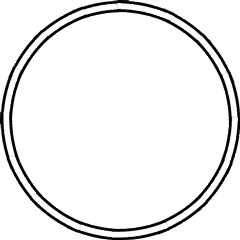
\includegraphics[height=1.2em]{images/0_1} \( 2_1 \):~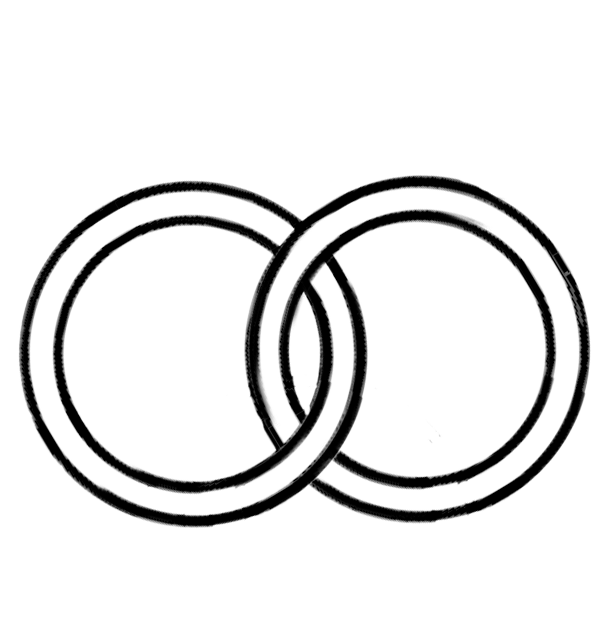
\includegraphics[height=1.2em]{images/hopf}\\
 \( 2_1 \):~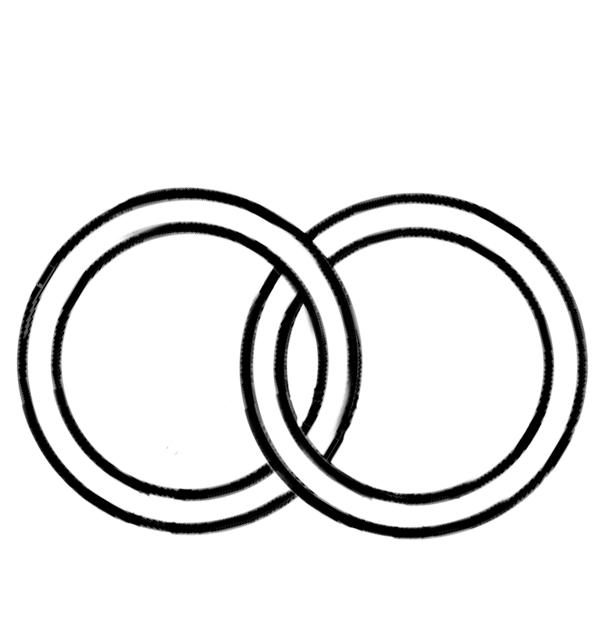
\includegraphics[height=1.2em]{images/ahopf}\\
 \( 2_1 \):~
\includegraphics[height=1.2em]{images/solomon}\\
 \( 2_1 \):~
\includegraphics[height=1.2em]{images/asolomon}\\
 \( 2_1 \):~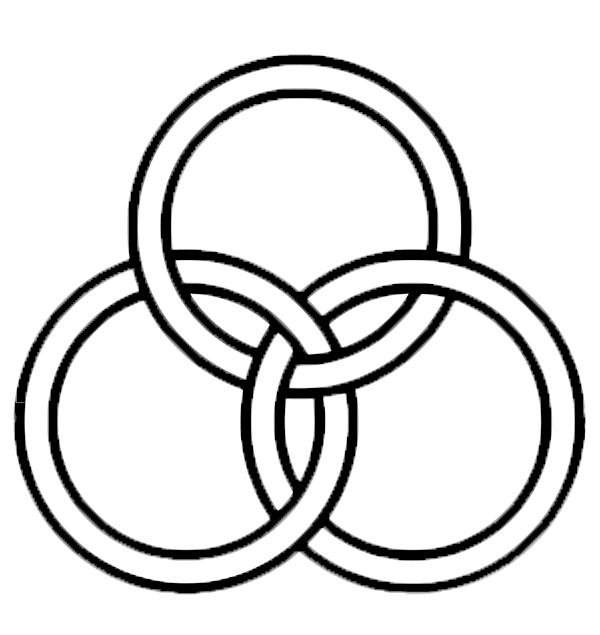
\includegraphics[height=1.2em]{images/borromean}\\
 \( 2_1 \):~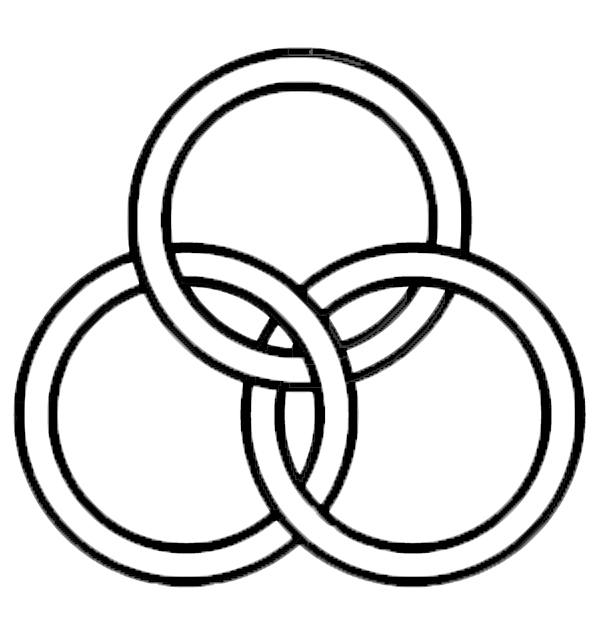
\includegraphics[height=1.2em]{images/aborromean}\\
 \( T(3,2) \):~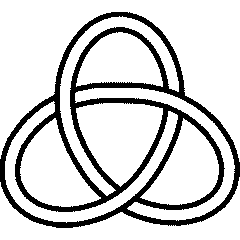
\includegraphics[height=1.2em]{images/3_1}\\
 \( T(2,3) \):~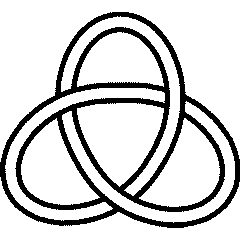
\includegraphics[height=1.2em]{images/a3_1}\\
 \( 6_2 \):~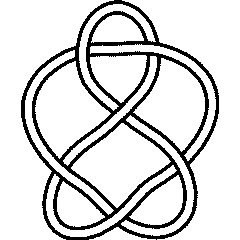
\includegraphics[height=1.2em]{images/6_2}\\
 \( 7_4 \):~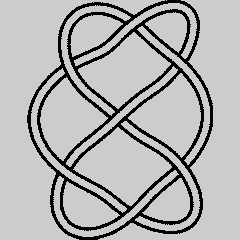
\includegraphics[height=1.2em]{images/7_4}\\
 \( 4_1 \):~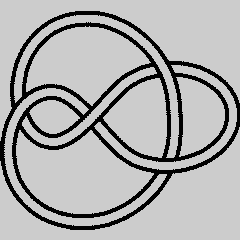
\includegraphics[height=1.2em]{images/4_1}
\begin{tikzpicture}[scale=0.1,  line width=0.4pt]
  \def\nsamples{60}
  \foreach \i in {1,...,\nsamples} {
      \pgfmathsetmacro\tprev{(\i - 1) * 2 * pi / \nsamples}
      \pgfmathsetmacro\tcurr{\i * 2 * pi / \nsamples}
      \pgfmathsetmacro\xprev{(2 + cos(2 * \tprev r)) * cos(3 * \tprev r)}
      \pgfmathsetmacro\yprev{(2 + cos(2 * \tprev r)) * sin(3 * \tprev r)}
      \pgfmathsetmacro\xcurr{(2 + cos(2 * \tcurr r)) * cos(3 * \tcurr r)}
      \pgfmathsetmacro\ycurr{(2 + cos(2 * \tcurr r)) * sin(3 * \tcurr r)}
      \draw[black, --] (\xprev,\yprev) -- (\xcurr,\ycurr);
  }
\end{tikzpicture}\\
 \( 5_1 \):~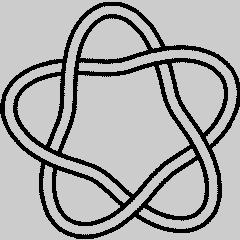
\includegraphics[height=1.2em]{images/5_1}\\
 \( 5_2 \):~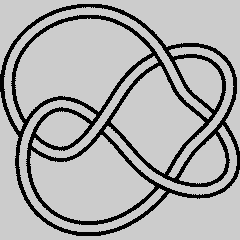
\includegraphics[height=1.2em]{images/5_2}\\
 \( 7_2 \):~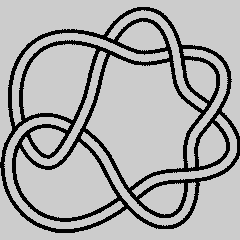
\includegraphics[height=1.2em]{images/7_2}\\




\section{Introduction and VAM Fundamentals}
The Vortex Æther Model (VAM) reformulates gravity and quantum phenomena as effects of vorticity in a 3D, Euclidean, inviscid Æther medium, rather than 4D spacetime curvature. In VAM, gravitation arises from vorticity-induced pressure gradients in a superfluid-like æther: intense vortex swirling creates Bernoulli-like low-pressure regions that act as gravitational potential wells. Time dilation likewise emerges from the energy and rotation of vortex structures (slower time in faster swirling regions),...

Fundamental Constants of VAM: The Æther medium is characterized by new constants that regulate its dynamics:
\begin{itemize}
    \item \textbf{$C_e$ (vortex tangential velocity constant)}: $C_e \approx 1.0938456\times10^6~\text{m/s}$, setting a characteristic speed for Æther circulation (comparable to $10^{-3}c$). This appears in vortex solutions and time dilation formulas as a limiting swirl speed.
    \item \textbf{$\rho_{\æ}$ (Æther density)}: $\rho_{\æ}$ is the mass density of the æther medium, estimated in VAM to lie between $5\times10^{-8}$ and $5\times10^{-5}~\text{kg/m}^3$. This extremely low density (comparable to cosmological vacuum density) allows the æther to sustain high vorticity with little inertia. It enters directly into gravitational and wave equations as the source of pressure gradients.
    \item \textbf{$F_{\max}$ (maximum Ætheric force)}: $F_{\max} \approx 29.05~\text{N}$ is an upper limit on force in the æther, analogous to the conjectured maximum force $c^4/4G$ in General Relativity. In VAM this emerges from vortex dynamics and the fine-structure constant, and will appear in wave propagation limits and nuclear scale analyses.
    \item \textbf{$r_c$ (vortex core radius / Coulomb barrier radius)}: $r_c \approx 1.40897\times10^{-15}~\text{m}$ is essentially a characteristic core size for vortices – on the order of a nucleon. It acts as a short-distance cutoff in VAM fields (preventing singularities) and represents the \grqq Coulomb barrier\textquotedblright radius inside which electrostatic/vortex forces sharply increase. No significant swirl can penetrate inside $r_c$ without enormous force, thus $r_c$ plays a central role in nuclear interactions.
    \item \textbf{$\kappa$ (vorticity conservation constant)}: $\kappa$ is a dimensionless constant ensuring quantization of vortex circulation. It appears in the energy of elementary vortex states, for example the quantized core energy $E_p = \kappa\,4\pi^2\,r_c\,C_e^2$. $\kappa$ can be chosen to fit known quantum energy scales (for instance, to recover an electron\rqs s orbital energy or rest energy), linking VAM\rqs s vortex model to observed particle values.
\end{itemize}

Using these constants, VAM replaces the usual fundamental constants ($c$, $G$, $\hbar$ in relativity/quantum theory) with fluid-like parameters ($C_e$, $\rho_{\æ}$, $\kappa$, etc.) that we will employ in deriving conditions for gravity modulation, FTL signaling, and LENR. The Æther is treated as an incompressible, non-viscous fluid supporting stable vortex filaments. All physical interactions are mediated by the dynamics of these vortices and pressure fields in the æther.

In the following sections, we develop a theoretical framework for:
\begin{enumerate}
    \item Manipulating gravity via topological vortex structures (including swirl shielding and frame-dragging effects),
    \item Enabling faster-than-light communication through ætheric wave channels,
    \item Triggering nuclear reactions via vortex-induced energy concentration and resonance.
\end{enumerate}
Each topic is grounded in VAM\rqs s equations and includes mathematical derivations and experimental proposals.


% ==================== Sections ====================

% ==================== Appendices ====================
\appendix

% ==================== Acknowledgments ====================
\section*{Acknowledgments}
The author thanks the online physics and alternative gravity communities for valuable discussions, and acknowledges support from the VAM open research initiative.

% ==================== References ====================
\bibliographystyle{apsrev4-2}
\bibliography{MASTER_references}

\end{document}
